
\begin{figure}
\hspace*{0mm}
\begin{tikzpicture}
  \node (template) {
    \begin{tikzpicture}
      \node[inner sep=0pt] (circuit) {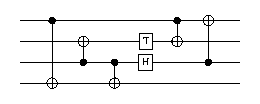
\includegraphics[scale=2]{Figures/circuits/vanillaCirc}};  
      \node[above left=8mm and -7mm of circuit.west, opacity=0.9] {\footnotesize \(A\)};
      \node[above left=1mm and -7mm of circuit.west, opacity=0.9] {\footnotesize \(B\)};
      \node[below left=1mm and -7mm of circuit.west, opacity=0.9] {\footnotesize \(C\)};
      \node[below left=8mm and -7mm of circuit.west, opacity=0.9] {\footnotesize \(D\)};
      \node[right=-3mm of circuit.north west, font=\itshape] (text) {a)};
    \end{tikzpicture}
  };
  \node[above right=-35.5mm and 6mm of template] (hypergraph) {
    \begin{tikzpicture}
      \coordinate (O) at (0,0);
      \coordinate (B) at (45:13mm);
      \coordinate (A) at (135:13mm);
      \coordinate (C) at (225:13mm);
      \coordinate (D) at (315:13mm);
      \coordinate (auxB) at (45:4.5mm);
      \coordinate (auxD) at (315:4.5mm);
      \draw (A) -- (C);
      \draw (A) -- (auxB);
      \draw (B) -- (auxB);
      \draw (D) -- (auxB);
      \draw (C) -- (auxD);
      \draw (B) -- (auxD);
      \draw (D) -- (auxD);
      \node[circle, right=-2.5mm of A, fill=white, inner sep=0pt, minimum size=5mm] {\(A\)};
      \node[circle, right=-2.5mm of B, fill=white, inner sep=0pt, minimum size=5mm] {\(B\)};
      \node[circle, right=-2.5mm of C, fill=white, inner sep=0pt, minimum size=5mm] {\(C\)};
      \node[circle, right=-2.5mm of D, fill=white, inner sep=0pt, minimum size=5mm] {\(D\)};
      \coordinate[above left=9mm and 1mm of O] (leftPoint);
      \coordinate[below left=9mm and 1mm of O] (rightPoint);
      \pic (cut) {cut=leftPoint/rightPoint};
      \node[above left=5mm and 9mm of A, font=\itshape] (text) {b)};
    \end{tikzpicture}
  };
  \node[below right=4mm and -92mm of template] (distributed) {
    \begin{tikzpicture}[transform canvas={scale=0.58}]
      \node[inner sep=0pt] (circuit) {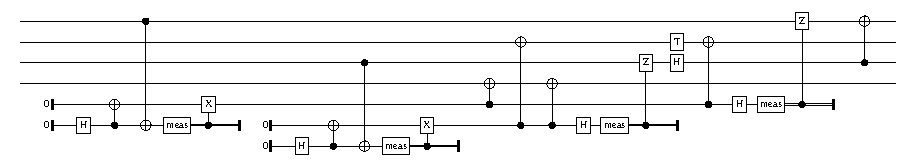
\includegraphics[scale=2]{Figures/circuits/vanillaDistrib}};
      \pic (e2) {ebitLong=e2/19.76mm/15.5mm};
      \pic (e1) {ebitLessClear=e1/26.8mm/16mm};
      \coordinate[left=-4mm of circuit.west] (leftPoint);
      \coordinate[right=-4mm of circuit.east] (rightPoint);
      \pic (cut) {cut=leftPoint/rightPoint};
      \node[above left=22mm and -7mm of circuit.west, opacity=0.9] {\(B\)};
      \node[above left=15mm and -7mm of circuit.west, opacity=0.9] {\(D\)};
      \node[below left=15mm and -7mm of circuit.west, opacity=0.9] {\(A\)};
      \node[below left=22mm and -7mm of circuit.west, opacity=0.9] {\(C\)};
    \end{tikzpicture}
  };
  \node[right=-1mm of distributed.north west, font=\itshape] (text) {c)};
\end{tikzpicture}
\vspace*{38mm}
\caption{The circuit is distributed using only \(2\) ebits. The other two possible distributions: \(\{\{A,B\},\{C,D\}\}\) and \(\{\{A,D\},\{B,C\}\}\) both require \(3\) ebits to be implemented. The wires in the distributed version of the circuit have been rearranged, so it is possible to visualise in a planar diagram that no quantum information crosses the boundary.}
\label{fig:vanillaExample}
\end{figure}
